\section{Definitions} \label{chapter3:definitions}

The continuous growth and sustainability of a platform relies on three criteria, Productivity, Efficiency and Adoption.
This section defines these tree criteria and their underlying concepts.

\subsection{Productivity} \label{chapter3:definitions:productivity}

The productivity of a platform is the degree to which developers can quickly produce new and modify existing software.
To support productivity, a platform needs to enforce modularity directly in the design of applications.
Productivity leads to maintainability.

Still, measuring productivity precisely to infer the improvement brought by a platform is highly difficult.
The measurement varies more between developers than between platforms \cite{Sackman1968}.

\subsubsection{Modularity} \label{chapter3:definitions:productivity:modularity}

Modularity is about encapsulating subproblems and composing them to allow greater design to emerge.
It allows to limit the understanding required to contribute to a module \cite{Stevens1974}.
% , which helps developers to repair and enhance the application. 
And it reduces development time by allowing developers to implement different modules simultaneously \cite{Wong2009,Cataldo2006}.

The criteria to define modules to improve productivity are high cohesion enforced by encapsulation and low coupling enforced by composition \cite{Stevens1974}.
Cohesion defines how strongly the features inside a module are related.
Coupling defines the strength of the interdependences between modules.

\separator

The criteria for productivity are the encapsulation and composition allowed by a platform.
Encapsulation relies on the definition of boundaries, and the protection of data.
Composition relies on higher-order programming and lazy evaluation.
The next paragraphs define these requirements.

\atomic {
  \begin{itemize}
  \item Encapsulation (Boundary definition, Data protection)
    \subitem $\to$ increases Cohesion
  \item Composition (Higher-order programming, Lambda Expressions) %, Lazy evaluation / Stream composition)
    \subitem $\to$ decreases Coupling
  \end{itemize}
}


\subsubsection{Encapsulation} \label{chapter3:definitions:productivity:encapsulation}

% \begin{wrapfigure}{R}{0.2\textwidth}
%   \centering
%   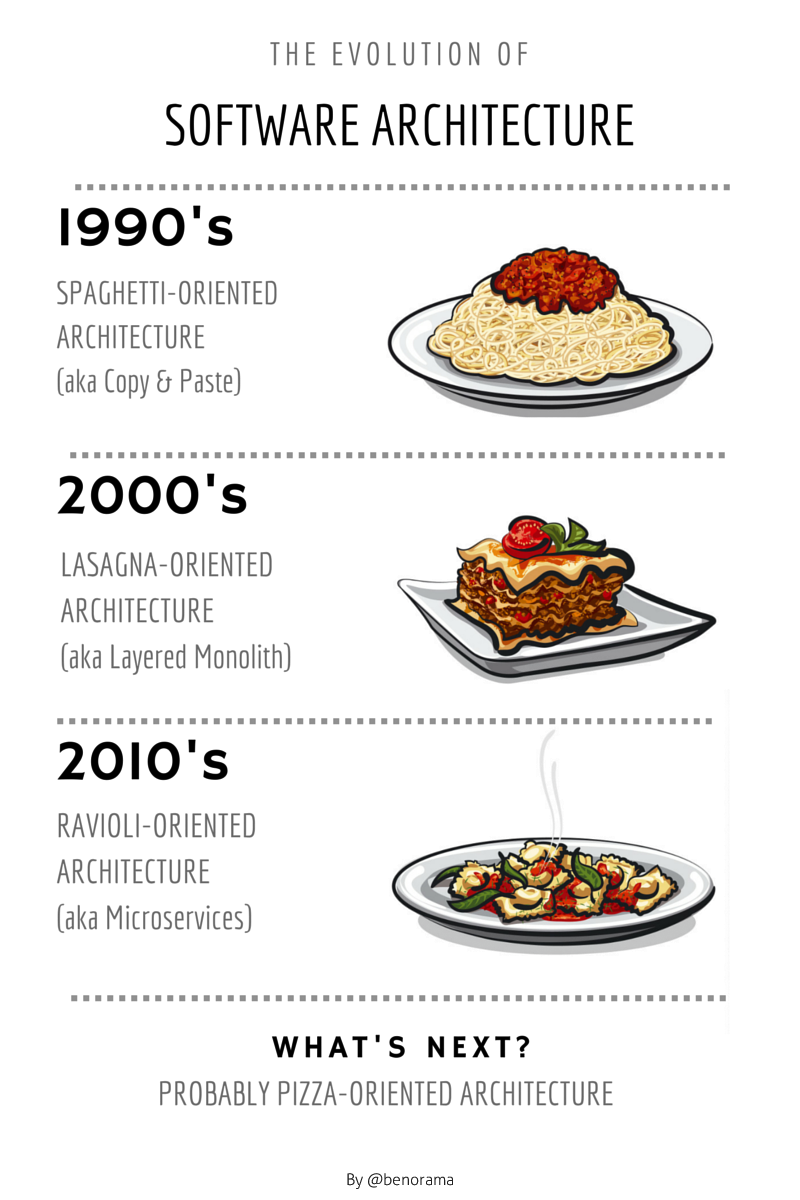
\includegraphics[height=0.1\textwidth]{../resources/italian-software-architecture.png}
% \end{wrapfigure}

\paragraph{Boundary Definition}
\illustration{spaghetti programming}%
Modular Programming draws clear interfaces around a piece of implementation so that the execution remains enclosed inside \cite{Dijkstra1970}.
At a fine level, it helps avoid spaghetti code \cite{Dijkstra1968a}, and at a coarser level, it structures the implementation \cite{Dijkstra1968} into modules, or layers.

\paragraph{Data Protection}
\illustration{lasagna programming}%
Modular programming encapsulates a specific design choice in each module, so that it is responsible for one and only one concern.
It isolates its evolution from impacting the rest of the implementation \cite{Parnas1972, Tarr1999, Hursch1995}.
Examples of such separation of concerns are the separation of the form and the content in HTML / CSS, or the OSI model for the network stack.

\subsubsection{Composition} \label{chapter3:definitions:productivity:composition}

\paragraph{Higher-Order Programming}
Higher-order programming introduces lambda expressions, functions manipulable like any other primary value.
They can be stored in variables, or be passed as arguments.
It replaces the need for most modern object oriented programming design patterns \ftnt{http://bit.ly/oop-patterns} with Inversion of Control \cite{Johnson}, the Hollywood Principle \cite{Sweet1985}, or Monads \cite{Wadler1992}.
Higher-order programming help loosen coupling, thus improve productivity \cite{Haynes1984}.

\paragraph{Closures}
In languages allowing mutable state, lambda expressions are implemented with closure to preserve the lexical scope \cite{Sussman1998}.
A closure is the association of a function and a reference to the lexical context from its creation.
It allows this function to access variable from this context, even when invoked outside the scope of this context.

% \paragraph{Lazy Evaluation}
% % Lazy evaluation 
% % Lazy evaluation is an evaluation strategy allowing to defer the execution of a function only when its result is needed.
% Lazy evaluation allows to defer the execution of an expression when its result is needed.
% The lazy evaluation of a list is equivalent to a stream with a null-sized buffer \cite{VanRoy2003}. %, while the opposite, eager evaluation, corresponds to an infinite buffer \cite{VanRoy2003}.
% It is a powerful tool for structuring modular programs, as the execution is organized as a concurrent pipeline \cite{Sussman1983}.
% The stages process independently each element of the stream.
% But this concurrency requires the isolation of side-effects to avoid conflicts between stages executions.
% % \nt{find another transition}Indeed, the dataflow programming paradigm resulting from lazy lists is particularly adapted for stream processing applications.

\subsection{Efficiency} \label{chapter3:definitions:efficiency}

The efficiency of a software project is the relation between the usage made of available resources and the delivered performances.
For an application to perform efficiently, its platform needs to enforce scalability directly in its design.

Scalability relies on the parallelism allowed by the commutativity of operations execution \cite{Clements2013a}.
An operation is a sequence of statements.
Operations are commutative if the order of their executions is irrelevant for the correctness of their results.
Commutativity assures the independence of operations.

\subsubsection{Independence} \label{chapter3:definitions:efficiency:independence}

\illustration{Synchronization vs Message-passing}
The independence, and commutativity of an operation depends on its accesses to shared state.
If the operation doesn't rely on any shared state, it is independent.
The independence of operations allows to execute them in parallel, hence to increase performance proportionally to occupied resources \cite{Amdahl1967,Gunther1993}.
But if they rely on shared state, they need to coordinate the causal scheduling and atomicity of their executions to avoid conflicting accesses.
This scheduling between the operations can be defined in two ways.
\begin{description}
\item[Synchronization] Operations are scheduled sequentially to have the exclusivity on a shared state, or
\item[Message-passing] Operations communicate their local modifications of the state to other operations as immutable messages.
\end{description}

Because of the latency associated with message-passing, the atomicity of operations is challenged.

\subsubsection{Atomicity} \label{chapter3:definitions:efficiency:atomicity}

An operation is atomic if it happens in a single bulk.
The beginning and end are indistinguishable for an external observer.
It assures the developer of the invariance of the memory during the operation.
It relies either on the causal scheduling of operations -- synchronization -- or exclusivity of their memory accesses -- message-passing.

\subsubsection{Granularity} \label{chapter3:definitions:efficiency:granularity}

If the operations access the state too frequently, the communication overhead of message passing exceeds the performance gains of parallelism.
Whereas if operations access the state too rarely, the synchronization required for sharing state limits the possible parallelism.
These two extremes are inefficient.
Operations tend to share state more closely at a fine-grain level and more loosely at a coarser-grain level.
Therefore, efficiency requires the combination of fine-level state sharing to avoid communication overhead, and coarse-level independence to allow parallelization \cite{Gustafson1988,Gunther1996,Nelson1996,Gunther2002}.
The threshold determining frequent or rare access to the state determines the granularity level between synchronization and parallelization of tasks.

\separator

The criteria to analyze the performance efficiency of platforms are the synchronization available at a fine-level, and the message-passing available at a coarse-level.

\atomic {
  \begin{itemize}
  \item Fine-level Synchronization
    \subitem $\to$ avoids communication overhead
  \item Coarse-level Message-passing
    \subitem $\to$ allows parallelism
  \end{itemize}
}

\subsection{Adoption} \label{chapter3:definitions:adoption}

An application is sustainable only if the platform used to build it generates reinforcing interactions between a community of passionate and the industry.
A platform needs to present a balance between productivity and efficiency to be adopted by both the community and the industry.
The productivity is required for a platform to be appealing to gather a community to support the ecosystem around it.
And the efficiency is required to be economically viable and needed by the industry, and to provide the reason for this ecosystem to exist.
The web acts as a tremendous catalyst fueling these interactions.

\separator

The criteria to analyze the adoption of platforms are the support of the community, and the industrial need.

\atomic {
  \begin{itemize}
  \item Community Support
    \subitem $\to$ grows an ecosystem
  \item Industrial Need
    \subitem $\to$ gives a goal for this ecosystem to grow
  \end{itemize}
}

\separator

Adoption requires a balance between efficiency and productivity.
This incentive to balance between productivity and efficiency is illustrated in figure \ref{fig:state-of-the-art}.
This figure is used throughout this chapter to graphically represent all the platforms analyzed.

\noindent
\dotcircled{1} references section \ref{chapter3:software-productivity:modularity}, the productivity focused platforms.\\
\dotcircled{2} references section \ref{chapter3:software-productivity:adoption}, their steering back toward efficiency.\\
\dotcircled{3} references section \ref{chapter3:software-efficiency:concurrency}, the efficiency focused platforms.\\
\dotcircled{4} references section \ref{chapter3:software-efficiency:adoption}, their steering back toward productivity.\\
\dotcircled{5} references section \ref{chapter3:software-adoption}, the platforms with a balance between productivity and efficiency.

\begin{figure}[h!]
\textfig{%
  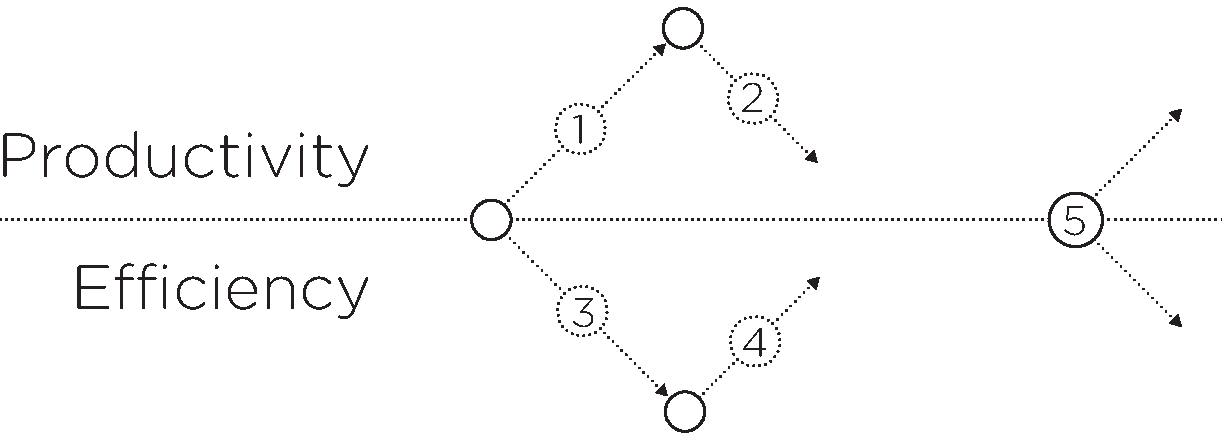
\includegraphics[width=0.6\textwidth]{../resources/state-of-the-art.pdf}%
  \caption{Balance between Efficiency and Productivity}%
  \label{fig:state-of-the-art}%
}%
\end{figure}